\documentclass[a4paper,11pt]{article}

\usepackage{url,amsmath,graphicx,booktabs,array,natbib,a4wide}
\usepackage{hyperref}
%\usepackage{Sweave}

\newcommand{\SGMplus}{AmpF\textit{l}STR\textsuperscript{\textregistered}
  SGM Plus\textsuperscript{\texttrademark}}

\newcommand{\proglang}[1]{\textsf{#1}}
\newcommand{\pkg}[1]{\textbf{#1}}
\newcommand{\code}[1]{\texttt{#1}}

\author{\begin{tabular}{c!{\hspace{10mm}}c}James M. Curran& Torben Tvedebrink \\University of
  Auckland& Aalborg University\end{tabular}}
\title{\pkg{DNAtools} : Tools for empirical testing of DNA match probabilities}
\date{}

\usepackage{color}
\definecolor{Blue}{rgb}{0,0,0.8}

\hypersetup{%
colorlinks,%
plainpages=true,%
linkcolor=black,%
citecolor=black,%
urlcolor=Blue,%
pdfstartview==FitW,%
pdfview={XYZ null null null},%
%pdfpagemode=UseNone,%
pdfauthor={James M. Currand and Torben Tvedebrink}%
}


\begin{document}

%\VignetteIndexEntry{Forensic genetics}
%\VignetteDepends{DNAtools}
%\VignetteKeywords{DNA databases}
%\VignettePackage{DNAtools}

%\SweaveOpts{engine=R,eps=FALSE}


\maketitle

\begin{abstract}
  DNA evidence is the pre-eminent tool in the modern forensic scientists
toolbox. It is widely accepted by the public, scientific and legal
communities and it has been instrumental in determining both the innocence
and guilt of individuals involved in the legal process. Despite this
widespread acceptance there
is unease regarding the statistical measures used to evaluate DNA
evidence amongst some of members of all these communities. In particular,
some people regard the random match probabilities associated with
DNA evidence as just too small or basically unsupportable. In this
article we discuss what it means for a pair of DNA profiles to match
or partially match, and we  present an \proglang{R} package that allows a rational
examination of the statistical properties of a DNA database.
\end{abstract}

\section[Introduction]{Introduction}
\label{sec:introduction}
In 2001, a poster was presented by a forensic scientist from Arizona
\citep{troyer2001} at a scientific meeting on human
identification. This poster reported a nine locus match between two
unrelated men, one white and one black \citep{kaye2009}.  It was not a
full match. Both men had been typed at thirteen loci in total, and
``partially matched'' at three of the remaining four loci. These
partially or non-matching loci would have excluded either man as a
suspect if the other was the true offender. However, such a match
seemed to be at odds with the random match probabilities. On one hand,
these two men were in a DNA database which consisted of approximately
65,000 profiles, and on the other hand, the random match probabilities
for the nine locus genotype were ``1 in 754 million in Caucasians, 1
in 561 billion in African Americans, and 1 in 113 trillion in
Southwest Hispanics'', \citet{troyer2001}.

As we will show later this is, in effect, an example of the ``birthday
problem'' and therefore is regarded as completely predictable from a
statistical perspective. However, most us who have taught a class on
the birthday problem know that our students are initially skeptical. 

\subsection[Matches and partial matches]{DNA evidence, matches and partial matches}
\label{sec:dna-matches-partial}
Forensic genetics has its terminology which we briefly explain here. 
Human DNA consists of 23 pairs of chromosomes and those
chromosomes are composed of a sequence of nucleotides which are
labeled A, G, C and T after the bases adenine, guanine, cytosine and
thymine that are used to form them. Modern DNA typing uses short
tandem repeats (STRs). These are regions of DNA which are highly
variable, but are patterned in that they consist of repeats of a short
sequence of DNA bases. The locations at which this information is
collected are called loci, and the (length) variations in the patterns
observed at each locus are called alleles. We have two alleles at each
locus, because humans are a diploid species, meaning they have two
copies of each chromosome. One allele comes from our mother, and the
other from our father. A pair of alleles at a locus is called a
genotype, and therefore a DNA profile is actually a multi-locus genotype.
Modern forensic laboratories genotype DNA evidence using commercial kits,
called multiplexes which consist of 9--17 loci. The multiplex currently
used in the United Kingdom (and until recently New Zealand and
Denmark) is called \SGMplus, or SGM Plus for short, and consists of 10 loci, plus one sex
specific locus, Amelogenin. Forensic laboratories in the United States
which load profiles into the FBI's Combined DNA Index System (CODIS) collect a
core set of thirteen loci, although they are not constrained to use
one multiplex.

\begin{table}[h]
  \centering
  \begin{tabular}{l*{10}{c}}
    \toprule
    Locus & vWA & D18 & TH01 & D2 & D8 & D3 & FGA & D16 & D21 & D19 \\
    \midrule
    Alleles & 15,18 & 14,17 &  6,9.3 & 17,23 & 12,15 & 15,15 & 19,23 & 11,12 & 28,28
    & 13,14\\
    \bottomrule
  \end{tabular}
  \caption{A DNA profile from the \SGMplus~multiplex}
  \label{tab:prof}
\end{table}

Table~\ref{tab:prof} shows a DNA profile from the \SGMplus~ multiplex.
There are two numbers at each locus representing the two alleles that
make up the genotype at that locus. The numbers relate to the number
of times the pattern or motif that describe the alleles at the locus
are repeated. For example, this person's genotype at the locus THO1 is
6,9.3. This means that on one chromosome, the motif for THO1,
\texttt{TCAT} was repeated 6 times, and on the other chromosome it was
repeated 9 times, and then followed by \texttt{TCA}. The .3 represents
the fact that three of the four bases have been repeated.

A pair of profiles is said to (fully) match if every allele at every
locus that occurs in one profile occurs in the other. A pair of
profiles are said to partially match if there are allelic matches at a
subset of loci.  \cite{weir2004} provided a taxonomy for describing
partial matches which depends on the number of fully, partial and
non-matching loci between a pair of profiles. For any given pair of
(full) profiles from the same multiplex there will be: $m_2$ loci
where both alleles match, $m_1$ loci where only one of the alleles
matches, and $m_0$ loci where none of the alleles match. For example,
the profile that \cite{troyer2001} found was a 9/3/1 partial match -
nine fully matching loci, three partially matching loci, and one
non-matching locus.

\subsection[Database comparisons]{DNA database comparison exercises}
\label{sec:dna-comp-exerc}
The Troyer match came from a database matching exercise. In such an
exercise every profile is compared with every other profile in the
database. This type of comparison exercise is absolutely essential
and, in addition, can provide some interesting information about the
statistical properties of the population under consideration. We say
that database comparison is essential in the first instance for the
detection of duplicates. Duplicates may arise in a number of different
ways. For example, an offender may provide a false name or an
offender's name may be entered incorrectly. Alternatively, an offender
may have an identical twin who is already in the DNA database. There
are six pairs of identical twins in the New Zealand National DNA
Database (NZDNADB). Forensic
scientists are also interested in 'very close' matches. 
For example, a pair of profiles
might fully match at nine loci out of ten and partially match at the
remaining locus. This may happen either because the donors of the
samples are very close relatives. It is  more likely, however, that
the profiles do not match because of allelic dropout,
primer binding site mutations, nomenclature changes or somatic mutation.

\subsection[The birthday problem]{The birthday problem}
\label{sec:are-numbers-wrong}
\cite{weir2007} and others \citep{brenner2007, curran2007,
  mueller2008, kaye2009} note that the presence of matching profiles
in a DNA database is effectively an instance of the well-known
``birthday problem'' \citep{wiki_birthday} where, in a group of at
least 23 randomly chosen people, there is a greater than 50\% chance
that one pair of them will have the same birthday. Early critics,
implicitly calculating the expected number of matches as $Np$, used
the wrong value for $N$ and the wrong value for $p$. Firstly, the
number of pairwise matches, not the size of the database, is the
relevant quantity. Although the database size is relatively small, the
number of pairwise comparisons is very large. The Arizona database
contained of $N=65,493$ profiles \citep{brenner2007}. Therefore,
there are
\[
N_\text{Comparisons}=\frac{N(N-1)}{2} = 2,144,633,778
\]
or approximately two billion, possible pairwise comparisons.
Secondly, the random match probability is not the probability we need.
The random match probability for the pair of profiles in question
answers the question ``What is the probability that someone other than
these two men would have this particular nine locus profile.'' The
probability we actually want is ``What is the probability that two
randomly selected profiles would match at nine loci, partially match
at three loci, and not match at one locus.''. \cite{weir2004},
working on an unrelated case, showed that this probability can be
calculated by
\begin{equation}
\label{eq:P}
P_{m_{0},m_{1},m_{2}}(\theta) = \sum_{m_{l0},m_{l1},m_{l2}}{\prod_l{P_{l2}(\theta)^{m_{l2}}P_{l1}(\theta)^{m_{l1}}P_{l0}(\theta)^{m_{l0}}}}
\end{equation}
where $m_{l0}$, $m_{1l}$ and $m_{l2}$ are indicator variables that are
equal to one if the individuals share zero, one or two alleles in
common respectively and zero otherwise. The expressions
$P_{li}(\theta)$ are the probability of sharing $i=0,1,2$ alleles in
common at locus $l$ for a given degree of population substructure
$\theta$ and are given explicitly in \cite{weir2004,weir2007}. The
coancestry coefficient, $\theta$ or $F_{ST}$ models low levels of
relatedness between individuals in the same subpopulation, and is
typically between 0 and 0.03.

\subsection[Modeling the data]{Modeling the observed data}
Weir's original paper \citep{weir2004} contained an informal analysis
where the minimum level of $\theta$ required to explain the observed
counts was calculated. For example using the FBI Caucasian data
\citep{budowle_1999} a $\theta$ value of 0.005 is needed to explain the
679 observed one locus matches (at locus FGA). That is, if
$\theta>0.005$, then the expected count at this locus will exceed the
observed count. \cite{curran2007} formalized and extended this
analysis in the following way. We model the expected number of pairs
of profile which fully match at $m_2$ loci and partially match at
$m_1$ loci for a given value of $\theta$, $E_{m_2/m_1}(\theta)$, as
\begin{equation*}
  \label{eq:1}
  E_{m_2/m_1}(\theta)=\alpha E_{m_2/m_1}^{U}(\theta)+ \beta
  E_{m_2/m_1}^{B}(\theta)+ \delta E_{m_2/m_1}^{C}(\theta)+ \gamma E_{m_2/m_1}^{P}(\theta)
\end{equation*}
where $0\le\alpha,\beta,\delta\le 1$ and
$\gamma=1-\alpha-\beta-\delta$. The quantities
$E_{m_2/m_1}^R(\theta),~ R\in\{U,B,C,P\}$ are the expected number of
matching pairs of profiles calculated under four relationship
categories: unrelated, full siblings (brothers), cousins, and
parent/child. These expressions are derived in \cite{curran2007},
with a typographical mistake corrected in
\citet{curran2010}. \citet{tvedebrink2010} also derived expressions
for avuncular relationships. \citet{curran2007} estimated
$\alpha,\beta,\delta,\gamma$ and $\theta$ by using a combination of a
line search (across $\theta$) and a Monte Carlo steepest descent
method to find the values that minimized several different distance
metrics applied to the observed and expected value. \citet{curran2007}
recommended minimizing
\begin{equation*}
  \label{eq:2}
  C_3(\theta) = \sum_{i=0}^{L}\sum_{j=0}^{L-m_2}\frac{|E_{i/j}(\theta)-O_{i/j}|}{O_{i/j}}
\end{equation*}
where $O_{i/j}$ is the observed number of pairs of profiles fully
matching at $m_2=i$ and $m_2=j$ loci using a multiplex consisting of
$L$ loci. This metric was chosen because of the belief that it puts
emphasis on ``explaining'' the higher order matches. Further research
into this by \citet{tvedebrink2010,tvedebrink2011} has shown that Mahalanobis
distance
\begin{equation*}
  \label{eq:3}
  T_2(\theta,) = \left(\vec{E}(\theta)-\vec{O}\right)^\top\Sigma(\theta)^{-}\left(\vec{E}(\theta)-\vec{O}\right)
\end{equation*}
actually provides a ``better'' fit to the data and does not drive the
value of $\theta$ to zero. $\Sigma(\theta)^{-}$ is a pseudo
inverse because of constraint
\[
\sum_{m_2=0}^{L}\sum_{m_1=0}^{L-m_2}P_{m_{2},m_{1},m_{0}}=1
\]

\section[DNAtools]{The \pkg{DNAtools} package}
The aim of the \pkg{DNAtools} package is to provide statisticians and
forensic scientists with access to the procedures described in the
previous sections. Early implementations by \cite{weir2004} and then
\cite{curran2007} required custom written code for each new database
and, in the case of \cite{curran2007}, generation of at least half a
dozen precursor files and a significant amount of memory.
\cite{tvedebrink2010,tvedebrink2011} reduced the computational
effort of \cite{weir2004} and \cite{curran2007} by deriving
recursion formulas for Equation \ref{eq:P}, improved the optimization
procedures through the use of the package \pkg{Rsolnp} \citep{Rsolnp},
and derived the variances of the probabilities which allowed both the
computation of Mahalanobis distances and asymptotic confidence
intervals. \pkg{DNAtools} aims to make all of these procedures easier
to use in \proglang{R} \citep{rcore2010}.

\section[Using DNAtools]{Using the package \pkg{DNAtools}}
\label{sec:package}

The expected data format of the databases used as input for the
functions in \pkg{DNAtools} is a data frame, which is constituted by a
column of DNA profile identifiers (the first column) and two columns
per typed DNA marker. An example is given below: 
\begin{verbatim}
head(get(data(dbExample)))[,1:9]
id D16S539.1 D16S539.2 D18S51.1 D18S51.2 D19S433.1 D19S433.2 D21S11.1 D21S11.2
 1        11        11       15       21        14        14       28       29
 2        13        12       15       14        16        16       29       28
 3         9         9       13       17        14        14       28       27
 4        11        12       14       15        15        13       32       29
 5        12        12       17       12      15.2        13     31.2       28
 6         9        13       17       14        13        14     30.2       28
\end{verbatim}

\cite{budowle_1999} published data from six US subpopulations of
different ethnicity (Caucasians, Hispanics, African Americans,
Bahamians, Jamaican and Trinidad). We demonstrate here our package
\pkg{DNAtools} using the Caucasian profiles typed at nine forensic STR
markers.

\begin{verbatim}
(caucasian.summary <- dbCompare(caucasian,hit=5))

Summary matrix
     partial
match    0    1    2    3    4    5    6    7    8    9
    0   17  145  628 1531 2416 2516 1822  752  170   26
    1   28  178  733 1426 1902 1455  727  211   40     
    2   13  121  303  530  492  310  108    9          
    3    5   32   64   99   52   23    6               
    4    0    6    6    7    2    1                    
    5    0    1    0    1    1                         
    6    0    0    0    0                              
    7    0    0    0                                   
    8    0    0                                        
    9    0                                             

Profiles with at least 5 matching loci
  ID1 ID2 match partial
1  10  29     5       4
2  77 116     5       3
3  64 170     5       1
\end{verbatim}

There is a \code{plot} method for the returned object. Applying this
method to \code{caucasian.summary} yields the ``dropping
ball''-picture of Figure~\ref{fig:caucasian}. The right end of the
``distribution'' is interesting part, due to the larger number of
coinciding loci between profile pairs.

\begin{figure}[!h]
  \centering
  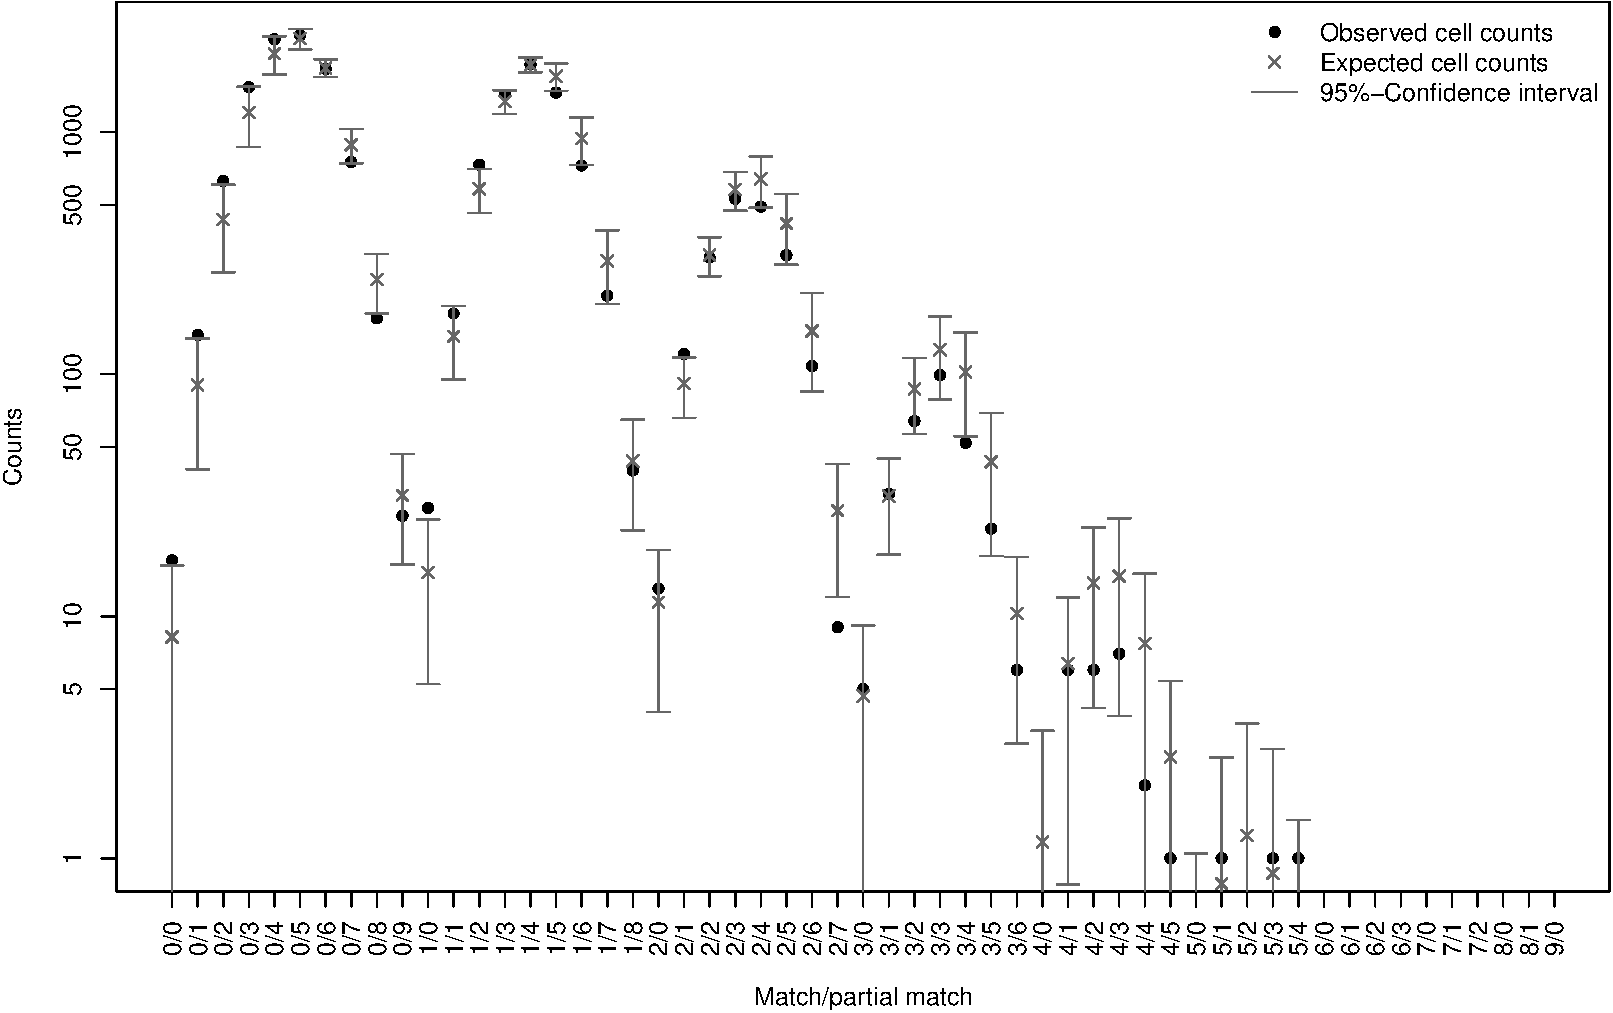
\includegraphics[width=15cm]{caucasianObsExp} % was : {plotCaucasianSummary}
  \caption{Plot produced by
    \code{plot(caucasian.summary,pch=16)}. Superimposed are the
    expected counts and associated 95\%-confidence intervals. The
    labels of the first axis denote the number of matching and
    partial-matching loci. The second axis is on a $\log_{10}$-scale.}
  \label{fig:caucasian}
\end{figure}

In Table~\ref{tab:caucasian}, the estimated parameters are reported
using the different object functions implemented in the
\code{optim.relatedness}-function of the
\pkg{DNAtools}-package. Only for $T_2$ the estimate of $\theta$ is
different from $0$.

\begin{table}
  \centering
  \begin{tabular}{>{$}l<{$}*{6}{r}}
    \toprule
    &$\theta$&Unrelated&First-Cousins&Avuncular&Parent-child&Full-siblings\\
    \midrule
    C_1&0&9.99e-01&2.32e-13&1.15e-08&5.01e-04&1.57e-04\\
    C_2&0&9.99e-01&6.90e-08&3.99e-08&1.16e-08&3.68e-14\\
    C_3&0&9.99e-01&2.16e-08&1.01e-11&1.08e-04&7.03e-04\\
    T_1&0&9.99e-01&3.97e-09&5.64e-12&4.63e-04&1.58e-05\\
    T_2&0.015&9.99e-01&1.67e-10&4.60e-06&7.47e-04&6.15e-06\\
    \bottomrule
  \end{tabular}
  \caption{\label{tab:caucasian}The estimated parameters of the model
    for the Caucasian sub\-sample.}
\end{table}

The fitted values can be used to compute $E_{m_2/m_1}(\theta)$. This
is done using \code{dbExpect} which takes $\theta$ and a list of locus
specific probability vectors as input. The function efficiently
computes the expectation using a recursion relation
\citep{tvedebrink2011}. Similarly, the superimposed confidence
intervals is Figure~\ref{fig:caucasian} were computed using the
\code{dbVariance}-function, which computes the covariance matrix of
the summary statistic \citep[also by recursion over
loci][]{tvedebrink2011}. The confidence intervals are based on a
normal approximation such that the width of the interval around the
expectations is computed as
$\pm2\sqrt{\text{diag}\{\Sigma(\theta)\}}$. This approximation is
asymptotic, hence the coverage accuracy decreases with the (expected)
cell count.

\paragraph{Availability}
\label{sec:software}

The \proglang{R}~package \pkg{DNAtools} is available at CRAN: 
\href{http://CRAN.R-project.org/package=DNAtools}{\pkg{DNAtools}}

\section[Conclusion]{Conclusion}
In this paper we have described an \proglang{R} package which allows
statisticians and forensic scientists to easily examine the properties
of a forensic DNA database. In particular, our package makes it simple
to carry out a database comparison exercise where every DNA profile in
the database is compared to every other database, and compare the
resulting numbers of observed pairs of matching and partially matching
profiles to expectation under a set of population genetic
assumptions. There are potential limitations on the use of this
package in that it may not scale well to extraordinarily large
databases ($>$100,000 profiles), but we expect that this will be
remedied by further development.

\section*{Acknowledgments}
We wish to acknowledge Professor Chris Triggs and the Department of
Statistics at the University of Auckland for financial support for
accommodation and travel for T.~Tvedebrink. We also wish to thank
Dr. John Buckleton for initially introducing us to this problem.
T.~Tvedebrink would like to thank Poul Svante Eriksen, Aalborg
University, for his contributions to the recursion formulas for
computing expectations and covariance matrices. 

\bibliographystyle{chicago}

\begin{thebibliography}{}
\newcommand{\enquote}[1]{``#1''}
\providecommand{\natexlab}[1]{#1}
\providecommand{\url}[1]{\texttt{#1}}
\providecommand{\urlprefix}{URL }
\expandafter\ifx\csname urlstyle\endcsname\relax
  \providecommand{\doi}[1]{doi:\discretionary{}{}{}#1}\else
  \providecommand{\doi}{doi:\discretionary{}{}{}\begingroup
  \urlstyle{rm}\Url}\fi
\providecommand{\eprint}[2][]{\url{#2}}

\bibitem[{Brenner(2007)}]{brenner2007}
Brenner C (2007).
\newblock \enquote{Arizona {DNA} Database Matches.}
\newblock Accessed 4-January-2010,
  \urlprefix\url{http://dna-view.com/ArizonaMatch.htm}.

\bibitem[{Budowle and Moretti(1999)}]{budowle_1999}
Budowle B, Moretti TR (1999).
\newblock \enquote{Genotype Profiles for Six Population Groups at the 13
  {CODIS} Short Tandem Repeat Core Loci and Other {PCR}-Based Loci.}
\newblock \emph{Forensic Science Communications}, \textbf{1}(2).
\newblock Accessed 5-January-2010,
  \urlprefix\url{http://www2.fbi.gov/hq/lab/fsc/backissu/july1999/budowle.htm}.

\bibitem[{Curran and Buckleton(2010)}]{curran2010}
Curran JM, Buckleton JS (2010).
\newblock \enquote{Re: Sign mistake in allele sharing probability formulae of
  {C}urran, et al.}
\newblock \emph{Forensic Science International: Genetics}, \textbf{4}(3),
  215--217.

\bibitem[{Curran \emph{et~al.}(2007)Curran, Walsh, and Buckleton}]{curran2007}
Curran JM, Walsh SJ, Buckleton J (2007).
\newblock \enquote{Empirical testing of estimated {DNA} frequencies.}
\newblock \emph{Forensic Science International: Genetics}, \textbf{1}(3-4),
  267--272.
\newblock ISSN 1878-0326.
\newblock \urlprefix\url{http://www.ncbi.nlm.nih.gov/pubmed/19083772}.

\bibitem[{Ghalanos and Theussl(2010)}]{Rsolnp}
Ghalanos A, Theussl S (2010).
\newblock \emph{\pkg{Rsolnp}: General Non-linear Optimization}.
\newblock \proglang{R}~package version~1.0-7,
  \urlprefix\url{http://CRAN.R-project.org/package=Rsolnp}.

\bibitem[{Kaye(2009)}]{kaye2009}
Kaye DH (2009).
\newblock \enquote{Trawling {DNA} Databases for Partial Matches: What Is the
  {FBI} Afraid Of?}
\newblock \emph{Cornell Journal of Law and Public Policy}, \textbf{19}(1), (in
  press).

\bibitem[{Mueller(2008)}]{mueller2008}
Mueller LD (2008).
\newblock \enquote{Can simple population genetic models reconcile partial match
  frequencies observed in large forensic databases?}
\newblock \emph{Journal of Genetics}, \textbf{87}(2), 101--108.
\newblock ISSN 0022-1333.
\newblock \urlprefix\url{http://www.ncbi.nlm.nih.gov/pubmed/18776637}.

\bibitem[{{R Development Core Team}(2010)}]{rcore2010}
{R Development Core Team} (2010).
\newblock \emph{R: A Language and Environment for Statistical Computing}.
\newblock R Foundation for Statistical Computing, Vienna, Austria.
\newblock {ISBN} 3-900051-07-0, \urlprefix\url{http://www.R-project.org}.

\bibitem[{Troyer \emph{et~al.}(2001)Troyer, Gilboy, and Koeneman}]{troyer2001}
Troyer K, Gilboy T, Koeneman B (2001).
\newblock \enquote{A nine {STR} locus match between two apparently unrelated
  individuals using {A}mp{F}\textit{l}{STR}\textsuperscript{\textregistered}
  {P}rofiler {P}lus\textsuperscript{\texttrademark} and
  {C}ofiler\textsuperscript{\texttrademark}.}
\newblock In \emph{Genetic Identity Conference Proceedings}, 12th International
  Symposium on Human Identification.
\newblock Accessed 4-January-2010,
  \urlprefix\url{http://www.promega.com/geneticidproc/ussymp12proc/abstracts/t%
royer.pdf}.

\bibitem[{Tvedebrink(2010)}]{tvedebrink2010}
Tvedebrink T (2010).
\newblock \emph{Statistical Aspects of Forensic Genetics -- Models for
  Qualitative and Quantitative STR Data}.
\newblock Ph.D. thesis, Department of Mathematical Sciences, Aalborg
  University.

\bibitem[{Tvedebrink \emph{et~al.}(2011)Tvedebrink, Eriksen, Curran, Mogensen, and Morling}]{tvedebrink2011}
Tvedebrink T, Eriksen PS, Curran JM, Mogensen HS, Morling N (2011).
\newblock \enquote{Analysis of matches and partial-matches in a Danish DNA
  reference profile data set.}
\newblock \emph{Forensic Science International: Genetics}.

\bibitem[{Weir(2004)}]{weir2004}
Weir BS (2004).
\newblock \enquote{Matching and partially-matching {DNA} profiles.}
\newblock \emph{Journal of Forensic Sciences}, \textbf{49}(5), 1009--1014.
\newblock ISSN 0022-1198.
\newblock \urlprefix\url{http://www.ncbi.nlm.nih.gov/pubmed/15461102}.

\bibitem[{Weir(2007)}]{weir2007}
Weir BS (2007).
\newblock \enquote{The rarity of {DNA} Profiles.}
\newblock \emph{The Annals of Applied Statistics}, \textbf{1}(2), 358--370.
\newblock ISSN 1941-7330.
\newblock \urlprefix\url{http://www.ncbi.nlm.nih.gov/pubmed/19030117}.

\bibitem[{Wikipedia(2010)}]{wiki_birthday}
Wikipedia (2010).
\newblock \enquote{Birthday problem.}
\newblock Accessed 5-January-2010,
  \urlprefix\url{http://en.wikipedia.org/wiki/Birthday_problem}.
\end{thebibliography}


\end{document}
